%%%%%%%%%%%%%%%%%%%%%%%%%%%%%%%%%%%%%%%%%%%%%%%%%%%%%%%%%%%%%%%%%%%%%%%%%%%%%%%%%%%%%%%%%%%%%%%%%%%%%%%%%%%%%%%%%%%%%%%%%%%%%%%%%%%%%%%%%%%%%%%%%%%%%%%%%%%%%%%%%%%%%%%%%%%%%%%%%%%%%%%%%%%%
% Written By Michael Brodskiy
% Class: Linear Algebra
% Professor: L. Knight
%%%%%%%%%%%%%%%%%%%%%%%%%%%%%%%%%%%%%%%%%%%%%%%%%%%%%%%%%%%%%%%%%%%%%%%%%%%%%%%%%%%%%%%%%%%%%%%%%%%%%%%%%%%%%%%%%%%%%%%%%%%%%%%%%%%%%%%%%%%%%%%%%%%%%%%%%%%%%%%%%%%%%%%%%%%%%%%%%%%%%%%%%%%%

\documentclass[12pt]{article} 
\usepackage{alphalph}
\usepackage[utf8]{inputenc}
\usepackage[russian,english]{babel}
\usepackage{titling}
\usepackage{amsmath}
\usepackage{graphicx}
\usepackage{enumitem}
\usepackage{amssymb}
\usepackage{physics}
\usepackage{tikz}
\usepackage{mathdots}
\usepackage{yhmath}
\usepackage{cancel}
\usepackage{color}
\usepackage{siunitx}
\usepackage{array}
\usepackage{multirow}
\usepackage{gensymb}
\usepackage{tabularx}
\usepackage{booktabs}
\usetikzlibrary{fadings}
\usetikzlibrary{patterns}
\usetikzlibrary{shadows.blur}
\usetikzlibrary{shapes}
\usepackage[super]{nth}
\usepackage{expl3}
\usepackage[version=4]{mhchem}
\usepackage{hpstatement}
\usepackage{rsphrase}
\usepackage{everysel}
\usepackage{ragged2e}
\usepackage{geometry}
\usepackage{fancyhdr}
\usepackage{cancel}
\usepackage{multicol}
\geometry{top=1.0in,bottom=1.0in,left=1.0in,right=1.0in}
\newcommand{\subtitle}[1]{%
  \posttitle{%
    \par\end{center}
    \begin{center}\large#1\end{center}
    \vskip0.5em}%

}
\usepackage{hyperref}
\hypersetup{
colorlinks=true,
linkcolor=blue,
filecolor=magenta,      
urlcolor=blue,
citecolor=blue,
}

\urlstyle{same}


\title{Linear Algebra 1.1 Homework}
\date{}
\author{Michael Brodskiy\\ \small Instructor: Prof. Knight}

% Mathematical Operations:

% Sum: $$\sum_{n=a}^{b} f(x) $$
% Integral: $$\int_{lower}^{upper} f(x) dx$$
% Limit: $$\lim_{x\to\infty} f(x)$$

\begin{document}

\maketitle

\begin{enumerate}

    \setcounter{enumi}{2}

  \item Not linear

    \setcounter{enumi}{4}

  \item Not linear

    \setcounter{enumi}{8}

  \item 

    \begin{equation*}
      \begin{split}
        y&\rightarrow s\\
        z&\rightarrow t\\
        S&=\left\{ (1-s-t,s,t) \right\}
      \end{split}
      \label{1}
    \end{equation}

  \item

    \begin{equation*}
      \begin{split}
        x_2&\rightarrow s\\
        x_3&\rightarrow t\\
        S&=\left\{ (1-2s+3t,s,t) \right\}
      \end{split}
      \label{2}
    \end{equation}

  \item \textbf{ }

    \begin{multicols}{2}

      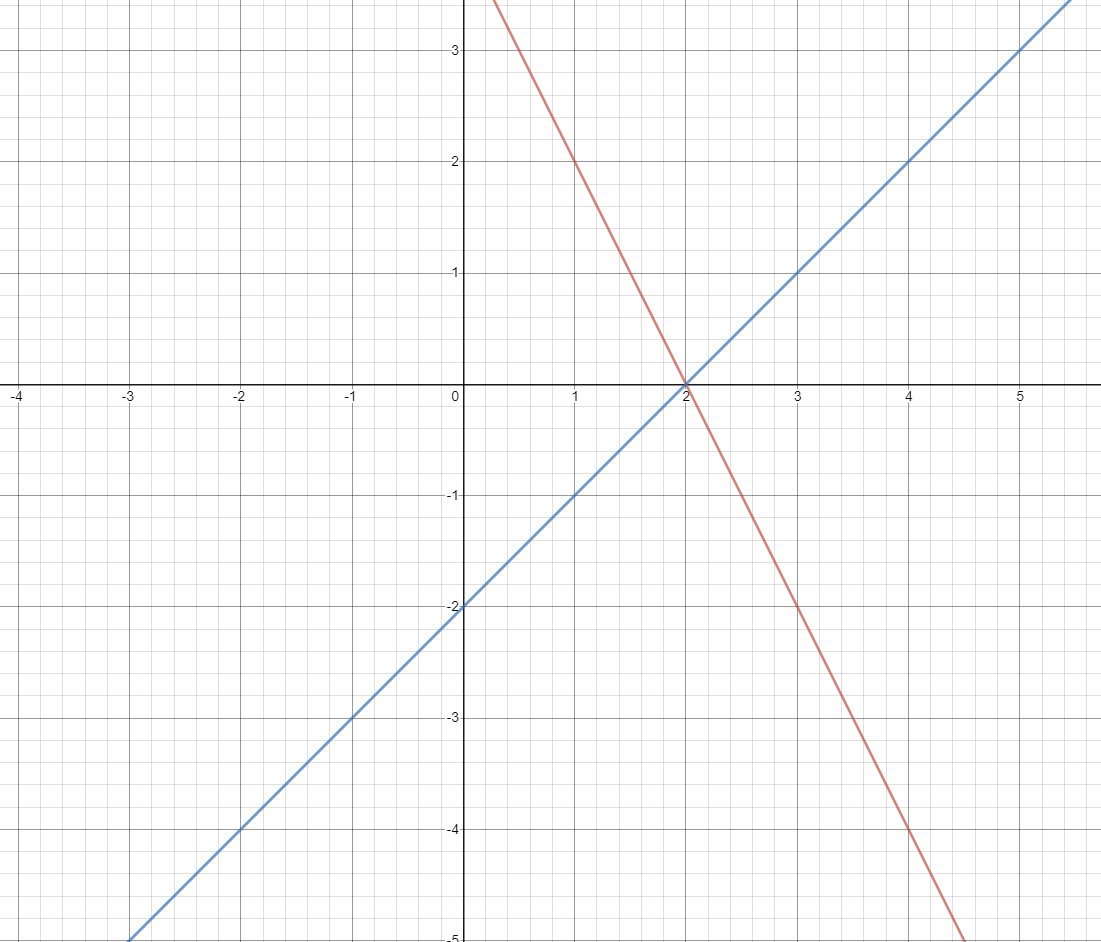
\includegraphics[width=.5\textwidth]{Figures/Prob11Graph.png}

    \begin{equation*}
      \begin{split}
        \begin{array}{l l}
          2x+y=4 & L_1\\
          x-y=2 & L_2
        \end{array}\\
        L_1-L_2\rightarrow x=2\\
        2(2)+y=4\\
        y=0\\
        \text{The solution is at point } (2,0)
      \end{split}
      \label{3}
    \end{equation}

  \end{multicols}

    \setcounter{enumi}{12}

  \item \textbf{ }

    \begin{multicols}{2}

      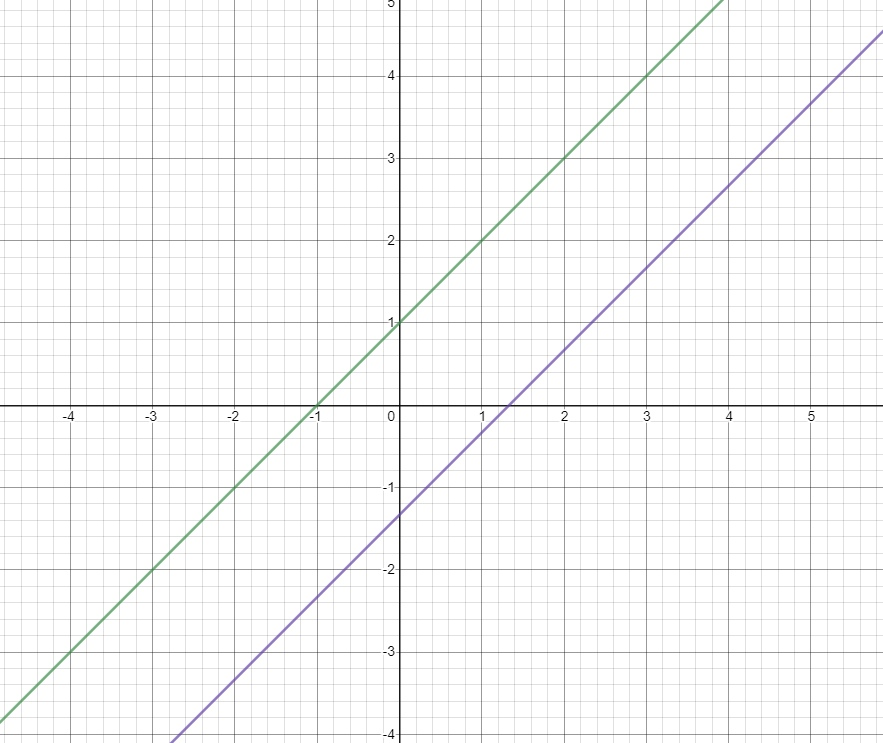
\includegraphics[width=.5\textwidth]{Figures/Prob13Graph.png}

    \begin{equation*}
      \begin{split}
        \begin{array}{l l}
          -x+y=1 & L_1\\
          3x-3y=4 & L_2
        \end{array}\\
        -\frac{1}{3}L_2\rightarrow -x+y=-\frac{4}{3}\\
        \text{No Solution, Lines Parallel}
      \end{split}
      \label{4}
    \end{equation}

  \end{multicols}

    \setcounter{enumi}{14}

  \item 

    \setcounter{enumi}{16}

  \item

    \setcounter{enumi}{18}

  \item

    \setcounter{enumi}{20}

  \item

    \setcounter{enumi}{22}

  \item

    \setcounter{enumi}{24}

  \item

    \setcounter{enumi}{26}

  \item

    \setcounter{enumi}{28}

  \item

    \setcounter{enumi}{38}

  \item

    \setcounter{enumi}{40}

  \item

    \setcounter{enumi}{46}

  \item

    \setcounter{enumi}{48}

  \item

    \setcounter{enumi}{50}

  \item

    \setcounter{enumi}{52}

  \item

    \setcounter{enumi}{64}

  \item

    \setcounter{enumi}{68}

  \item

    \setcounter{enumi}{70}

  \item

    \setcounter{enumi}{74}

  \item

    \setcounter{enumi}{76}

  \item

    \setcounter{enumi}{78}

  \item

    \setcounter{enumi}{80}

  \item

    \setcounter{enumi}{82}

  \item

    \setcounter{enumi}{84}

  \item

\end{enumerate}

\end{document}

